\documentclass[11pt,a4paper]{article}

\newcommand{\tumsoTime}{09:00 น. - 12:00 น.}
\newcommand{\tumsoRound}{1}

\usepackage{../tumso}

\usepackage{soul}

\begin{document}

\begin{problem}{Cargo Container}{standard input}{standard output}{0.75 seconds}{64 megabytes}{75}

ในโลกของเรามีตู้คอนเทนเนอร์ขนสินค้าอยู่ถึงมากกว่า 65 ล้านตู้คอยหมุนเวียนขนสินค้าไปรอบ ๆ โลกของเรา เช่น ตู้ขนของเล่นที่ผลิตด้วยแรงงานเด็กจากประเทศโลกที่ 3 มาให้เด็กประเทศโลกที่ 1 เล่น
\begin{figure}[htp]
    \centering
    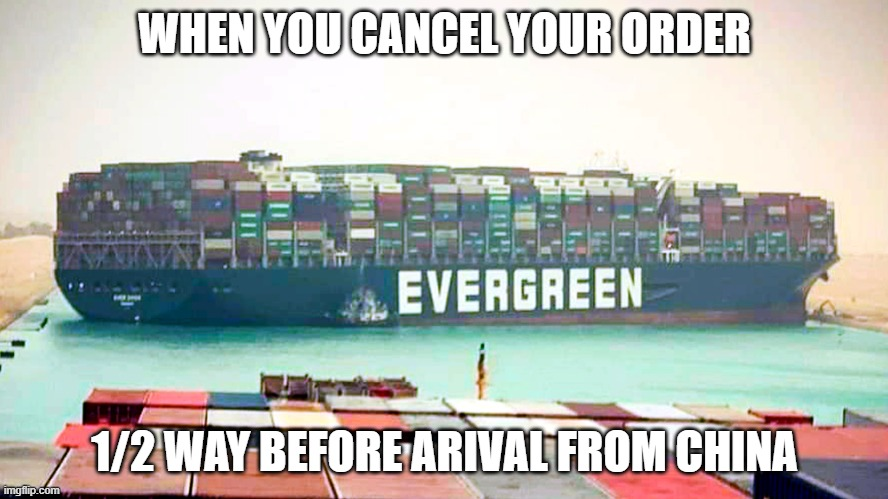
\includegraphics[width=8cm]{cargocontainercheck/Evergreen.jpg}
    \caption{ภาพตู้คอนเทนเนอร์บนเรือสินค้า}
\end{figure}

โดยตู้คอนเทนเนอร์ทุกตู้จะมีรหัส ID ไม่ซ้ำกันอยู่ 11 ตัวอักษรเสมอ เช่น TEMU6284450 โดยรหัสจะประกอบไปด้วย 4 องค์ประกอบได้แก่

\begin{enumerate}
    \item Owner Prefix 3 ตัวแรกของชื่อตู้จะบอกบริษัทเจ้าของตู้ TEM (TEXTAINER EQUIPMENT MANAGEMENT LTD)
    \item Equipment Identifier ตัวอักษรตัวที่ 4 จะบอกประเภทของตู้ U (Freight Container) J (Detachable frieght container) etc.
    \item Serial Number ตัวเลขที่ 5 ถึง 10 ของตู้ เพราะฉะนั้นเจ้าของจะสามารถมีเลขตู้ได้ถึงคนละ 1 ล้านตู้
    \item Check Digit ตัวเลขตัวสุดท้ายโดยคำนวณมาจาก ตัวเลข/ตัวอักษร ที่ 1-10 เพื่อช่วยในการยืนยันความถูกต้องของชื่อตู้
\end{enumerate}

\begin{figure}[htp]
    \centering
    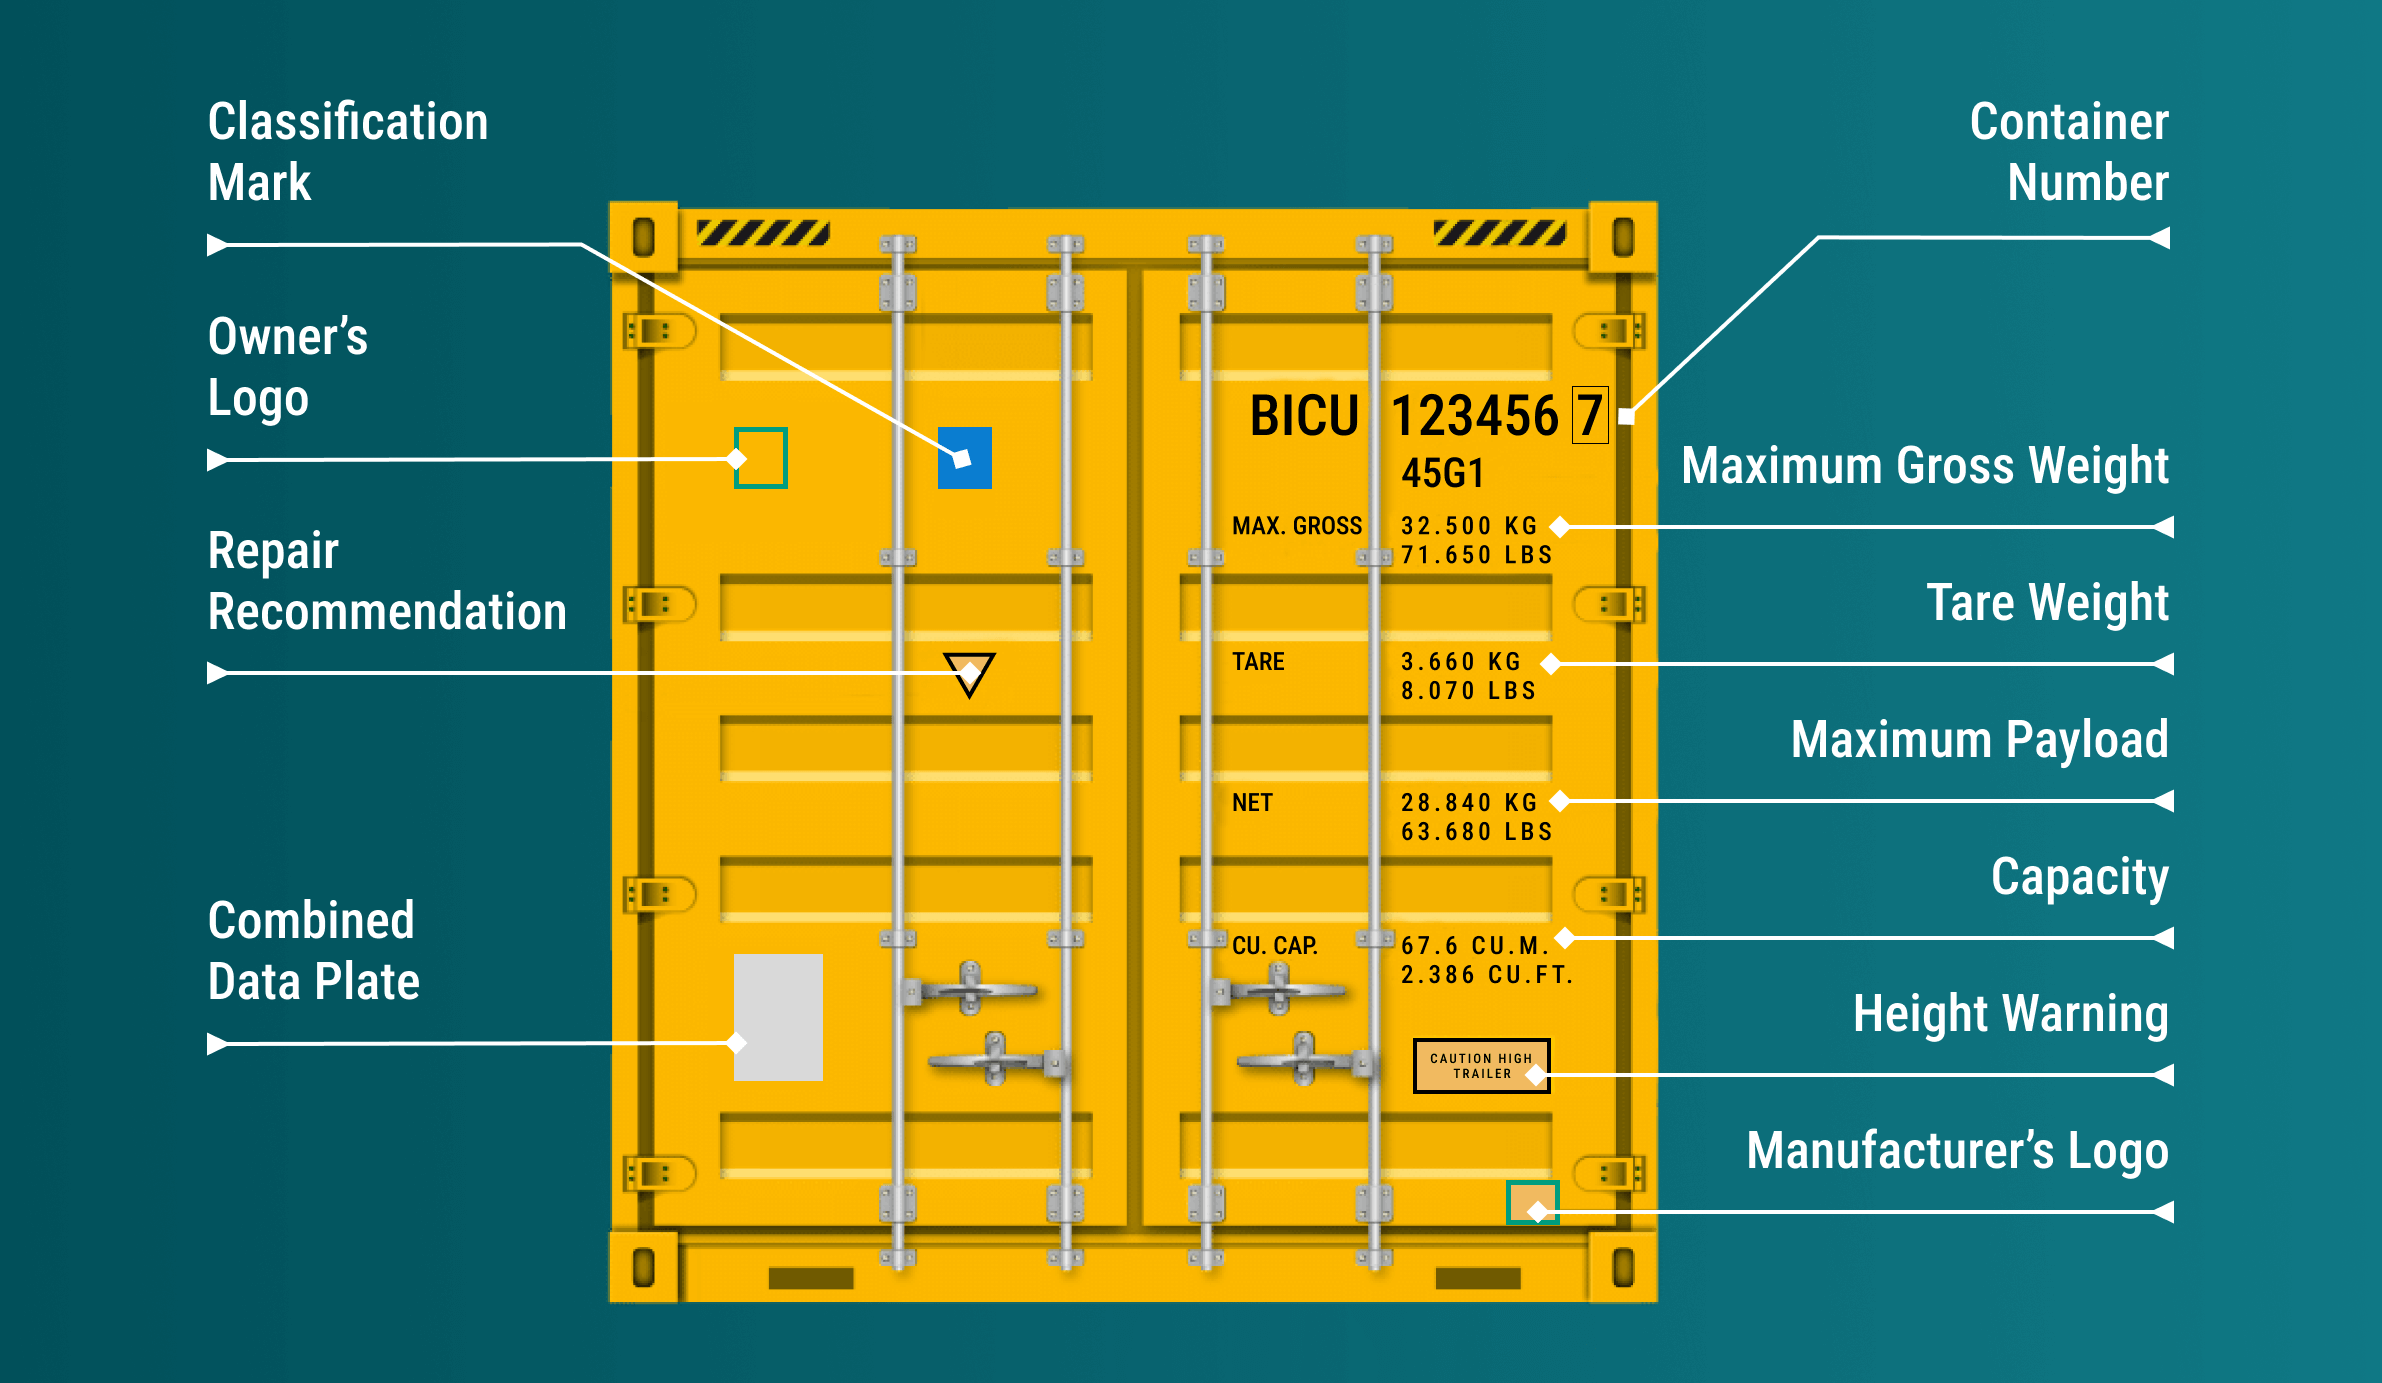
\includegraphics[width=8cm]{cargocontainercheck/Container-Markings-1-1.png}
    \caption{รายละเอียดอื่นๆบนตู้คอนเทนเนอร์}
\end{figure}

นายอทิณัทฐ์ ปราโมทย์ ได้รับคำสั่งจากหัวหน้างานให้ตรวจสอบตู้คอนเทนเนอร์จำนวน 500 ตู้ว่าชื่อตู้มีความถูกต้องไหมแต่นายอทิณัทฐ์ ขี้่เกียจที่จะนั่งคำนวณด้วยมือนายอทิณัทฐ์จึงต้องการที่จะเขียนโปรแกรมตรวจสอบอัตโนมัติแต่เมื่อนำไปเสนอหัวหน้าหัวหน้าได้ต่อว่าว่าทำเรื่องไร้สาระจึงไล่นายอทิณัทฐ์ ออกจากงานของเขาทำให้นายอทิณัทฐ์ไม่สามารถหาเงินมาใช้หนี้สิ้นได้จึงโดนมาเฟียเก็บอวัยวะไปขายได้แก่

\begin{enumerate}
    \item ไตข้างซ้าย
    \item ปอดข้างขวา
\end{enumerate}

แต่ในความจริงเนื่องจากหัวหน้างานชอบไอเดียของนายอทิณัทฐ์มาก แต่ไม่ต้องการจ่ายค่าจ้างจึงทำการ Out Source งานไปที่ Syria ให้นาย Abu Hajaar ทำงานนี้ให้และนาย Abu Hajaar ก็ Out Source ให้น้องทำงานนี้ให้โดยเข้าได้มอบวิธีการคำนวณ Check Digit ให้น้อง

โดยในขั้นตอนแรก ทุก ๆ อักขระ latin จะมีค่ากำกับดังในตารางต่อไปนี้ ส่วนตัวเลขจะมีค่าตามตัวเลข
\begin{figure}[htp]
    \centering
    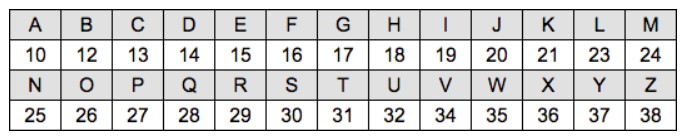
\includegraphics[width=12cm]{cargocontainercheck/value.jpg}
\end{figure}

ในขั้นตอนต่อไปเราจะกำหนดค่าด้วยตารางให้ตัวอักษรที่ 1-10 เพื่อคำนวณหาตัวอักษรที่ 11 หรือ Check Digit

\begin{figure}[htp]
    \centering
    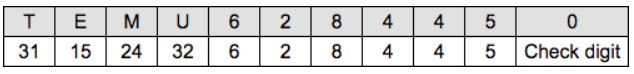
\includegraphics[width=12cm]{cargocontainercheck/assigned.jpg}
\end{figure}

ในขั้นตอนต่อไปเราจะ คูณ ค่าที่ได้ของแต่ละตำแหน่งด้วย 2 ยกกำลังตำแหน่ง แล้วหาผลรวมทั้งหมด

\begin{figure}[htp]
    \centering
    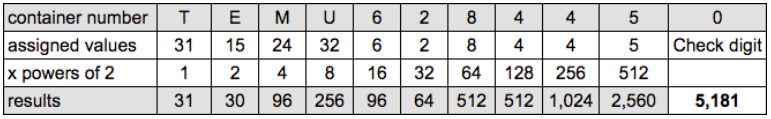
\includegraphics[width=12cm]{cargocontainercheck/power.png}
    \end{figure}
\newpage

หารค่าที่ได้ด้วย 11 โดยปัดทศนิยมลงเสมอ 5181 หารด้วย 11 ค่าที่เราต้องการคือ 471 จากนั้นนำตัวเลขที่ได้ออกมาคูณด้วย 11 แล้วผลต่างของเลขตอนต้นกับท้ายคือ Check Digit ของเรานั้นเอง ถ้าหาก Check Digit คำนวณได้ 10 ให้ถือว่า Check Digit มีค่าเท่ากับ 0

\begin{figure}[htp]
    \centering
    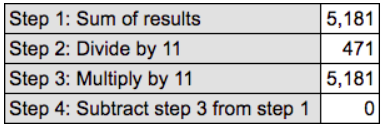
\includegraphics[width=8cm]{cargocontainercheck/final.png}
\end{figure}

\InputFile

% ข้อมูลนำเข้ามีทั้งหมด $N$ บรรทัด โดยแต่ละบรรทัดประกอบไปด้วย ID ตู้คอนเทนเนอร์ (ไม่มีตัวซ้ำ)

ข้อมูลนำเข้ามีทั้งหมด $Q+2$ บรรทัด

บรรทัดแรกประกอบด้วยจำนวนเต็ม $N$ แทนจำนวนตู้คอนเทนเนอร์ $(1\leq N\leq 10^{5})$

อีก $N$ บรรทัดประกอบด้วยสายอักขระ $S$ แทน ID ของตู้คอนเทนเนอร์ $(|S|=11)$

รับประกันว่าอักขระตัวที่ 1 ถึง 4 จะเป็นตัวอักษร A ถึง Z และอักขระตัวที่ 5 ถึง 11 จะเป็นตัวเลขเสมอ

\textbf{คำเตือน} ชื่อตู้คอนเทนเนอร์อ่านโดยคนที่สายตาสั้น 900 จึงไม่สามารถตัดเลนส์สำหรับ Oculus Quest 3 ได้ เพราะฉะนั้นอาจเกิดความผิดพลาดในการอ่านได้

\OutputFile
มีไม่เกิน $N$ บรรทัด ตามจำนวนตู้คอนเทนเนอร์ที่มีความถูกต้อง โดยเรียงตามลำดับของข้อมูลนำเข้า

\Scoring
คะแนนเต็มในข้อนี้คือ 75 คะแนน โดยจะได้คะแนนตามสัดส่วนของชุดทดสอบที่ตอบได้ถูกต้อง คะแนนที่ได้ในข้อนี้คือคะแนนในการส่งครั้งที่ดีที่สุด

\Examples

\begin{example}
\exmp{5
TEMU6284450
TGHU7599330
PFXU5088331
TEMU3214342
PFXU5023331
}{TEMU6284450
TGHU7599330
PFXU5088331
}%
\end{example}

\end{problem}

\end{document}
